\documentclass{beamer}

\usetheme{Padova}

\title{Componente di controllo per l'elaborazione in tempo reale di flussi di dati aggregati}
%\subtitle{Curabitur sit amet mi magna}
\author{Niccolò Mantovani}
\date{30 Settembre 2021}


\begin{document}

	\maketitle

	\begin{frame}{Outline}
		\tableofcontents
	\end{frame}


	\section{L'azienda}

	\begin{frame}{L'azienda}

		\textbf{Datasoil s.r.l.} \vspace{.2em}
		
		\textit{Startup} Innovativa fondata nel 2016 come \textit{Open Innovation} nell’ambito delle aziende manifatturiere. \vspace{.2em}
		
		\begin{itemize}
			\item \textit{Software as a Service} in \textit{cloud} \textbf{B2B} e \textbf{B2C} \vspace{.5em}
			\item Analisi, elaborazione e fruizione di dati \vspace{.5em}
			\item Piattaforma proprietaria \textbf{SYN}
		\end{itemize}
		
		\begin{figure}[!h] 
    		\centering 
    		
\includegraphics[width=0.2\columnwidth]{../immagini/ds_logo.png}
		\end{figure}

	\end{frame}

	\section{Il progetto}

	\begin{frame}{Il progetto}
	\vspace{.5em}
		Creazione di una componente aggiuntiva per la piattaforma \textbf{SYN}. \vspace{.2em}
		
		\begin{block}{Obiettivi}
			\begin{itemize}
				\item Elaborazione \textit{streaming} di eventi provenienti da \textbf{risorse differenti} \vspace{.5em}
				\item Raggruppamento temporale \vspace{.5em}
				\item Raggruppamento secondo caratteristiche specifiche \vspace{.5em}
				\item Rilevazione di anomalie \vspace{.5em} 			
			\end{itemize}
		\end{block}
		
		\begin{figure}[!h] 
    		\centering 
    		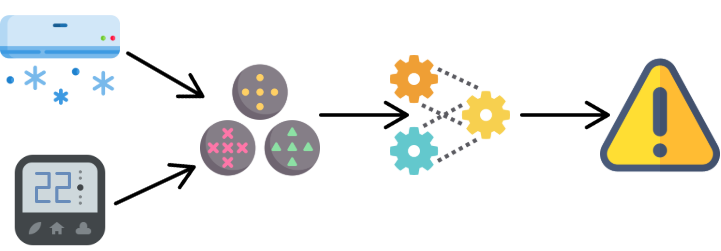
\includegraphics[width=0.55\columnwidth]{../immagini/slide/elaboration_example.png}
		\end{figure}
		
	\end{frame}
	
	\subsection{Problema affrontato}

	\begin{frame}{Problema affrontato}

		\begin{alertblock}{Adattabilità struttura dati}
			Rappresentazione di eventi facenti parte di un \textbf{gruppo} \vspace{.5em}
		\end{alertblock} \vspace{.2em}
		
		\begin{alertblock}{Adattabilità raggruppamento}
			\begin{itemize}
				\item Temporale su eventi di \textbf{risorse differenti} \vspace{.5em}
				\item Per caratteristiche su eventi di \textbf{risorse differenti} \vspace{.5em}
			\end{itemize}
		\end{alertblock}
		
		\begin{alertblock}{Adattabilità rilevazione anomalie}
			Rilevazione di anomalie e produzione di \textit{alert} su \textbf{gruppi} di eventi \vspace{.5em} 
		\end{alertblock}
	\end{frame}
	
	\subsection{Soluzione proposta}

	\begin{frame}{Soluzione proposta}
		\begin{exampleblock}{Adattabilità struttura dati}
			Proin tincidunt, neque at tincidunt mollis
		\end{exampleblock}
		
		\begin{exampleblock}{Adattabilità raggruppamento}
			Proin tincidunt, neque at tincidunt mollis
		\end{exampleblock}
		
		\begin{exampleblock}{Adattabilità rilevazione anomalie}
			Proin tincidunt, neque at tincidunt mollis
		\end{exampleblock}
	\end{frame}
	
	\section{Implementazione}

	\begin{frame}{Implementazione}
		\begin{block}{Normal block}
			Fusce luctus venenatis felis quis semper
		\end{block}

		\begin{alertblock}{Alert block}
			$$ E = (x_1 \vee \neg x_2 \vee \neg x_3) \wedge (x_1 \vee x_2 \vee x_4) $$
		\end{alertblock}

		\begin{exampleblock}{Example block}
			Proin tincidunt, neque at tincidunt mollis
		\end{exampleblock}
	\end{frame}
	
	\section{Strumenti utilizzati}

	\begin{frame}{Strumenti utilizzati}
		\begin{block}{Framework}
			\begin{itemize}
				\item \textbf{Flink:} \textit{data processing} per l'elaborazione di dati in modo distribuito \vspace{.5em}
				\item \textbf{ScalaTest:} stesura dei test relativi all'analisi effettuata da \textit{Flink} \vspace{.5em}
			\end{itemize}
		\end{block}
		
		\begin{block}{Linguaggi di programmazione}
			\begin{itemize}
				\item \textbf{Scala:} utilizzato tramite \textit{Flink} \vspace{.5em}
				\item \textbf{Go:} utilizzato per le \textit{API} \vspace{.5em}
			\end{itemize}
		\end{block}
	\end{frame}
	
	\subsection{Flink}
	\begin{frame}{Flink}
	
	\end{frame}
	
	\section{Prodotto finale}

	\begin{frame}{Prodotto finale}
		\begin{block}{Normal block}
			Fusce luctus venenatis felis quis semper
		\end{block}

		\begin{alertblock}{Alert block}
			$$ E = (x_1 \vee \neg x_2 \vee \neg x_3) \wedge (x_1 \vee x_2 \vee x_4) $$
		\end{alertblock}

		\begin{exampleblock}{Example block}
			Proin tincidunt, neque at tincidunt mollis
		\end{exampleblock}
	\end{frame}
	
	\section{Considerazioni}

	\begin{frame}{Considerazioni}
		\begin{block}{Normal block}
			Fusce luctus venenatis felis quis semper
		\end{block}

		\begin{alertblock}{Alert block}
			$$ E = (x_1 \vee \neg x_2 \vee \neg x_3) \wedge (x_1 \vee x_2 \vee x_4) $$
		\end{alertblock}

		\begin{exampleblock}{Example block}
			Proin tincidunt, neque at tincidunt mollis
		\end{exampleblock}
	\end{frame}
	
	\subsection{Possibili miglioramenti}

	\begin{frame}{Possibili miglioramenti}
		\begin{block}{Normal block}
			Fusce luctus venenatis felis quis semper
		\end{block}

		\begin{alertblock}{Alert block}
			$$ E = (x_1 \vee \neg x_2 \vee \neg x_3) \wedge (x_1 \vee x_2 \vee x_4) $$
		\end{alertblock}

		\begin{exampleblock}{Example block}
			Proin tincidunt, neque at tincidunt mollis
		\end{exampleblock}
	\end{frame}
	
	\subsection{Conoscenze acquisite}

	\begin{frame}{Conoscenze acquisite}
		\begin{block}{Normal block}
			Fusce luctus venenatis felis quis semper
		\end{block}

		\begin{alertblock}{Alert block}
			$$ E = (x_1 \vee \neg x_2 \vee \neg x_3) \wedge (x_1 \vee x_2 \vee x_4) $$
		\end{alertblock}

		\begin{exampleblock}{Example block}
			Proin tincidunt, neque at tincidunt mollis
		\end{exampleblock}
	\end{frame}


\end{document}
